\documentclass{ximera}
\title{Mean Value Theorem}
\begin{abstract}
\end{abstract}
\begin{document}
\maketitle

\section{Introduction}

\begin{dialogue}
\item[Dylan] I don't know about this theorem...it seems pretty \textit{mean}...
\item[Julia] No no, they mean \textit{mean} as in average!
\item[Dylan] Oh, so were looking at the average value of a function?
\item[James] Not quite, actually the \textbf{mean value theorem} states the following: If $f$ is continuous on $[a,b]$ and differentiable on $(a,b)$, then there exists at least one value $c$ in $(a,b)$ such that $$f'(c)=\frac{f(b)-f(a)}{b-a}$$
\item[Dylan and Julia] Maybe we should do an example...that looks pretty confusing...
\item[ALTOGETHER] Let's dive in!
\end{dialogue}

\section{Guided Example}

Take a look at the following graph illustrating the Mean Value Theorem:

\begin{image}
    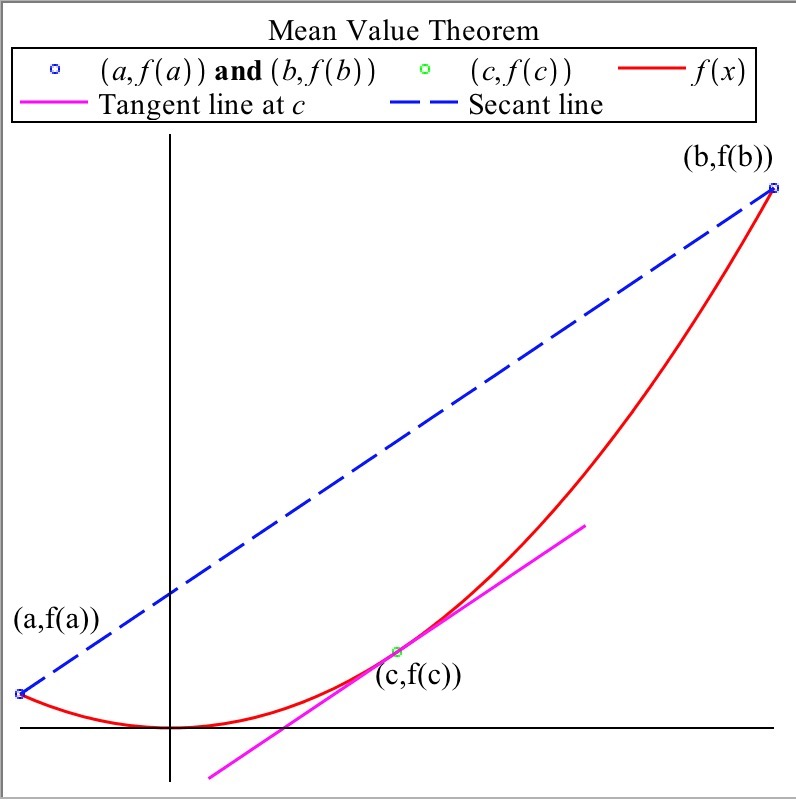
\includegraphics[width=80mm]{meanvalue.jpg}
\end{image}

\begin{question}
What do you notice about the tangent line at $c$ with respect to the secant line from $a$ to $b$?

\begin{multipleChoice}
\choice[correct]{They are parallel.}
\choice{The slope of the tangent line is half that of the secant line.}
\choice{The tangent line is perpendicular to the secant line.}
\choice{The tangent line intersects the secant line.}
\end{multipleChoice}

What does this mean the derivative of $f(x)$ is at $c$?

\begin{multipleChoice}
\choice{$\frac{1}{2}$}
\choice{$\frac{a-b}{f(a)-f(b)}$}
\choice[correct]{$\frac{f(b)-f(a)}{b-a}$}
\choice{$\frac{2a}{b}$}
\end{multipleChoice}

If $f'(x)$ was zero for all points in the interval, what could always be said about $f(x)$ on that interval?
\begin{multipleChoice}
\choice{$f(x)$ is positive at all points on the interval.}
\choice{$f(x)$ is negative at all points on the interval.}
\choice[correct]{$f(x)$ is a constant on the interval.}
\choice{$f(x)$ does not exist on the interval.}
\end{multipleChoice}
\begin{explanation}
Let $a< b$ be two points in $I$. Since $f$ is continuous on $[a,b]$
and differentiable on $(a,b)$, by the Mean Value Theorem we know
\[
\frac{f(b)-f(a)}{b-a} = f'(c)
\]
for some $c$ in the interval $(a,b)$. Since $f'(c)=0$ we see that
$f(b)=f(a)$. Since $a$ and $b$ were arbitrarily chosen,
$f(x)$ must be constant on the interval.
\end{explanation}
\end{question}
\begin{question}
Use $f(x)=\sin(2x)$ on the interval $[0,2\pi]$ for the following questions.
\begin{hint}
To graph $f(x)=\sin(2x)$ on the domain $[0,2\pi]$ in desmos type: sin(2x){0<=x<=2pi}.
\end{hint}
Graph $f(x)$
\[
\graph{}
\]

What values for $c$ satisfy the mean value theorem?(figure out where the derivative equals the slope of the secant line!)

\begin{selectAll}
\choice[correct]{$\frac{\pi}{4}$}
\choice{$1$}
\choice{$\frac{3\pi}{5}$}
\choice[correct]{$\frac{3\pi}{4}$}
\choice[correct]{$\frac{5\pi}{4}$}
\choice{$0$}
\choice{$\pi$}
\choice[correct]{$\frac{7\pi}{4}$}
\end{selectAll}

\end{question}

\section{On Your Own}
Let $f(x)=\left|x^2-x-2\right|$.
\[
\graph{f(x)=abs(x^2-x-2)}
\]


\begin{question}
Examine the graph. Does the function satisfy the hypothesis of the Mean Value Theorem on the interval $[a,b]=[0,3]$?

\begin{multipleChoice}
\choice{Yes}
\choice[correct]{No}
\end{multipleChoice}

\end{question}

\begin{question}
Consider $f(x) = \frac{1}{x}$.
\[
\graph{1/x}
\]

Over which of the following regions does the function satisfy the hypothesis of the Mean Value Theorem?

\begin{selectAll}
\choice{$[-10,10]$}
\choice{$[0,10]$}
\choice[correct]{$[1,10]$}
\choice[correct]{$[-10,-1]$}
\choice{$[-10,0]$}
\end{selectAll}

Apply the Mean Value Theorem from [1, 4], determining what points experience the same instantaneous change as the entire interval.
$\answer{\frac{2}{\sqrt{3}}}$
\end{question}

\begin{question}
Seeing a police officer on the side of the road, your friend Tom slows down to 35 mph. However, once the officer pulls over someone else for speeding, Tom speeds up to 70 mph. Half an hour and 35 miles later, Tom checks his navigation app and sees another police officer is up ahead, slowing himself down to the legal 35 mph. However, the police officer still pulls Tom over, saying he had been radioed by the first officer right when Tom passed, so he could prove that Tom was going 70 mph at some point in the last half hour. Tom is furious about the clearly faulty reasoning of the police officer. Let $g(x)$ be the position of Tom's car at time $x$.

Thanks to the Mean Value Theorem, you know that the police officer is in the right. Using $g(x)$, explain to Tom why the officer had a valid reason to ticket him.
\begin{hint}
What would Tom's average speed have to be to get 35 miles in a half hour?
\end{hint}

\begin{freeResponse}
\end{freeResponse}

Talking to Tom, you find out that he accelerated to 70 mph in only 5 seconds after passing the officer. Prove that at some point, Tom had an acceleration of over 25,000 $\text{mi} \backslash \text{h}^2$.
\begin{hint}
What would Tom's average change of velocity have to be to go from 35 mph to 70 mph in 5 seconds(make sure to convert the seconds to hours)?
\end{hint}
\begin{freeResponse}
\end{freeResponse}
\end{question}

\section{In Summary}

\begin{theorem}
The \textbf{Mean Value Theorem} states that for any function $f$, if $f$ is continuous on $[a,b]$ and differentiable on $(a,b)$, then there exists at least one value $c$ such that $$f'(c)=\frac{f(b)-f(a)}{b-a}$$

This means that there is a point $c$ such that the secant line from $a, b$ has the same slope as the tangent line at $c$. It's important to note that this means if $f'(x)=0$ for all $x$ on $(a,b)$, then $f$ is constant on $(a,b)$.
\end{theorem}
\end{document}